\section{Flujo de trabajo para el versionamiento de cursos}
\begin{table}[H]
\centering
\caption{Historias de usuario para el flujo de trabajo para el versionamiento de cursos}
\label{epic:6}
\resizebox{\columnwidth}{!}{%
\begin{tabular}{@{}llllll@{}}
\toprule
Historias de usuario              & HE & HC & PH & PA & CS \\ \midrule
Versionamiento de cursos          & 84 & 96 & 13 & 8 & 2 \\
Información básica de curso       & 46 & 53 & 5 & 1 & 1 \\
Horas y unidades de evaluación    & 48 & 66 & 5 & 0 & 1 \\
Especificaciones de curso         & 40 & 40 & 5 & 2 & 1 \\
Requisitos de curso               & 44 & 40 & 5 & 3 & 1 \\
Revisar y aprobar curso           & 48 & 68 & 5 & 2 & 1 \\
Competencias de curso             & 80 & 76 & 8 & 2 & 1 \\
Esquema de curso                  & 40 & 48 & 5 & 1 & 1 \\
Códigos de clasificación de curso & 56 & 80 & 5 & 3 & 1 \\ \bottomrule
\end{tabular}
}
\end{table}


\subsection{Versionamiento de cursos}
Esta historia de usuario fue realizada en tres iteraciones con un total de 96 horas cargadas, debido a que los cambios que suponía conlleva a una migración importante de datos de los usuarios.

Tenía como descripción los siguiente \enquote{\textit{Como coordinador del AMS, me gustaría poder hacer una versión de mi plan de curso para que pueda realizar un seguimiento de los cambios para cosas como la revisión de programas y los acuerdos de articulación y transferencia en la aplicación}}.

Algunas de las tareas realizadas en la historia fueron las siguientes:

\begin{itemize}
	\item Buscar técnicas y herramientas de versionamiento parecidas para implementar.
	\item Diseñar una posible solución a la problemática.
	\item Implementar cambios en la base de datos mediante scripts en el proyecto.
	\item Actualizar clases de Java existentes en el proyecto de cursos.
	\item Implementar la solución para el flujo de trabajo.
	\item Actualizar la creación de cursos sin el módulo curricular con los nuevos campos.
	\item Adaptar la relación de cursos y competencias para que soporte el versionamiento de los mismos.
	\item Actualizar la lista de competencias por cursos.
\end{itemize}

\subsection{Información básica de curso}
Esta historia de usuario tiene como propósito de diseñar páginas que permitan al usuario completar la información básica de curso que buscan diseñar, así también fueron proporcionados mockups para la pantalla (figura \ref{course_cover_info}).

Tiene la siguiente descripción: \enquote{\textit{Como miembro del comité de Curriculum, me gustaría ser capaz de administrar la página de información básica de cursos, para que no tenga que buscar por documentos a la hora de crear o versionar cursos}}.

\begin{itemize}
	\item Diseñar un modelo de datos que soporte el nuevo formato de información de curso.
	\item Adaptar tablas existentes y crear clases nuevas para las nuevas entidades de base de datos.
	\item Actualizar la plantilla de creación de Workflow para que soporte el nuevo paso.
	\item Actualizar el visualizador de Workflow.
	\item Diseño de pruebas automatizadas.
\end{itemize}

La historia se terminó en una iteración con un total de 53 horas de desarrollo.

\begin{figure}[H]
\centering
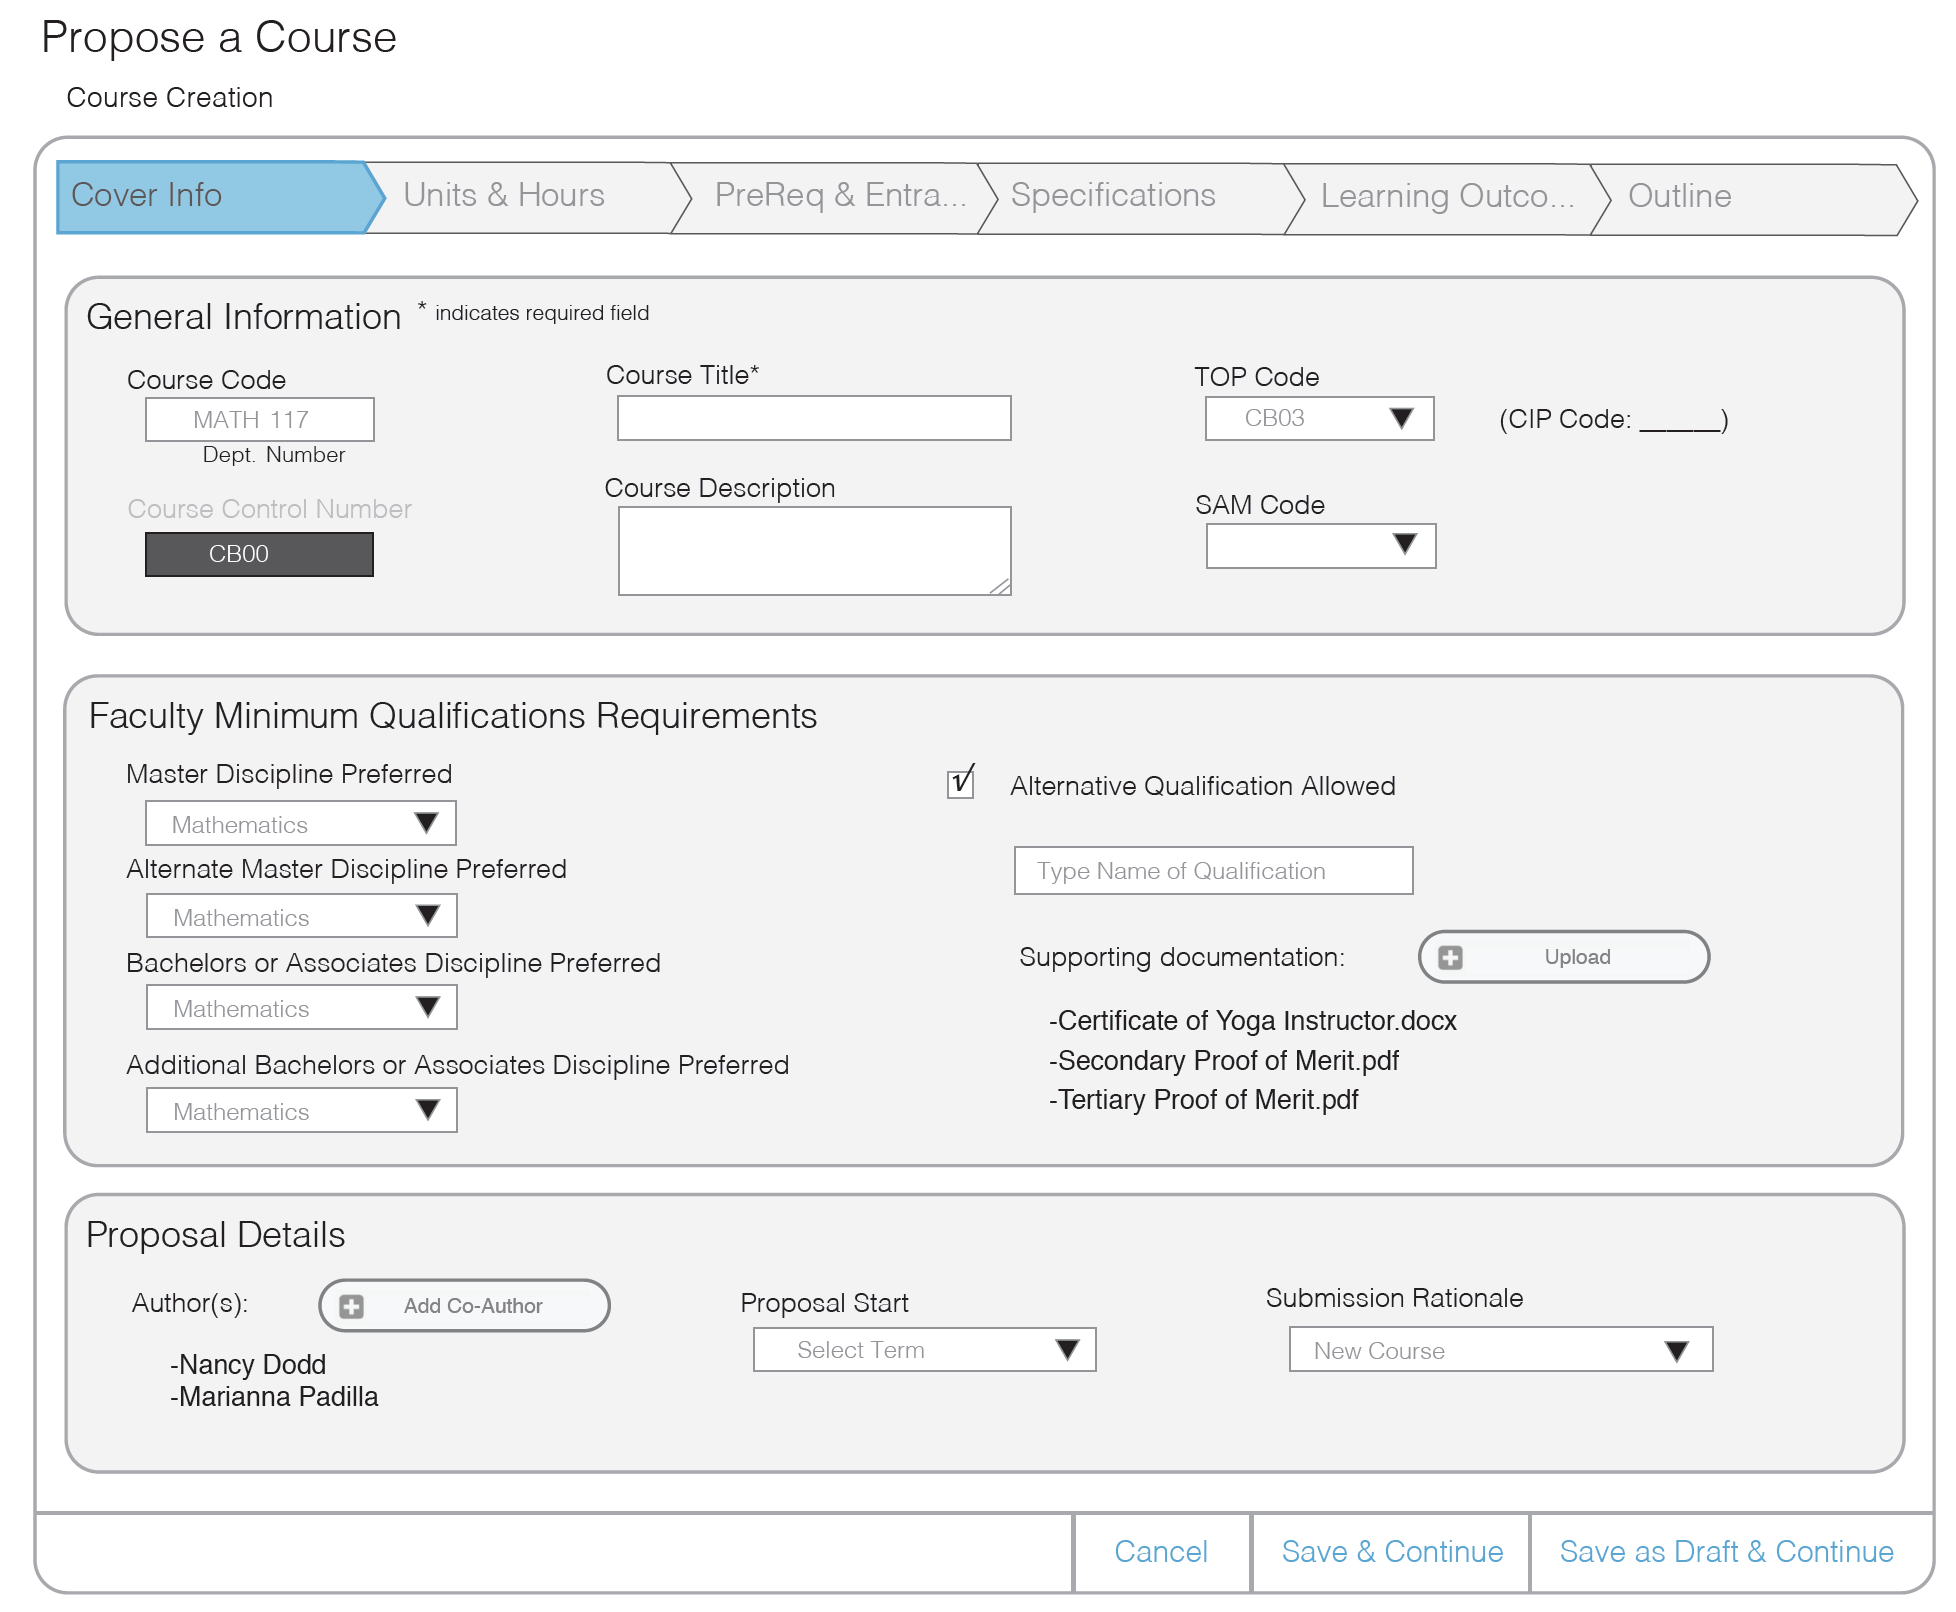
\includegraphics[scale=0.3]{Capitulos/DesarrollodelaAplicacion/Imagenes/course_cover_info}
\caption{Mockup de la pantalla de información básica de curso.}
  \label{course_cover_info}
\end{figure}

\subsection{Horas y unidades de evaluación}
En esta historia se desarrolló un nuevo paso para el desarrollo de flujo de trabajo, en la cual el encargo del mismo va a poder detallar las horas y unidades que requiere el curso o que va a requerir.

La organización ha proveído mockups (figura \ref{course_units_hours}) para la página como criterio de aceptación de la historia es que siga el modelo de la misma.

La historia tenía la siguiente descripción: \enquote{\textit{Como profesor encargado del curso, me gustaría tener una página de horas y métricas para que pueda conseguir información básica sobre mi curso en eLumen}}.

La historia a desarrollar se dividió entre miembros del equipo de desarrollo en las siguientes tareas:
\begin{itemize}
	\item Modificar el modelo de datos para que soporte los nuevos campos de curso.
	\item Crear y/o editar las clases Java.
	\item Actualizar la plantilla de flujo de trabajos.
	\item Actualizar el visualizador de flujo de trabajos.
	\item Pruebas de funcionalidad.
\end{itemize}

La historia ha sido terminada en una iteración con un total de 66 horas de desarrollo.

\begin{figure}[H]
\centering
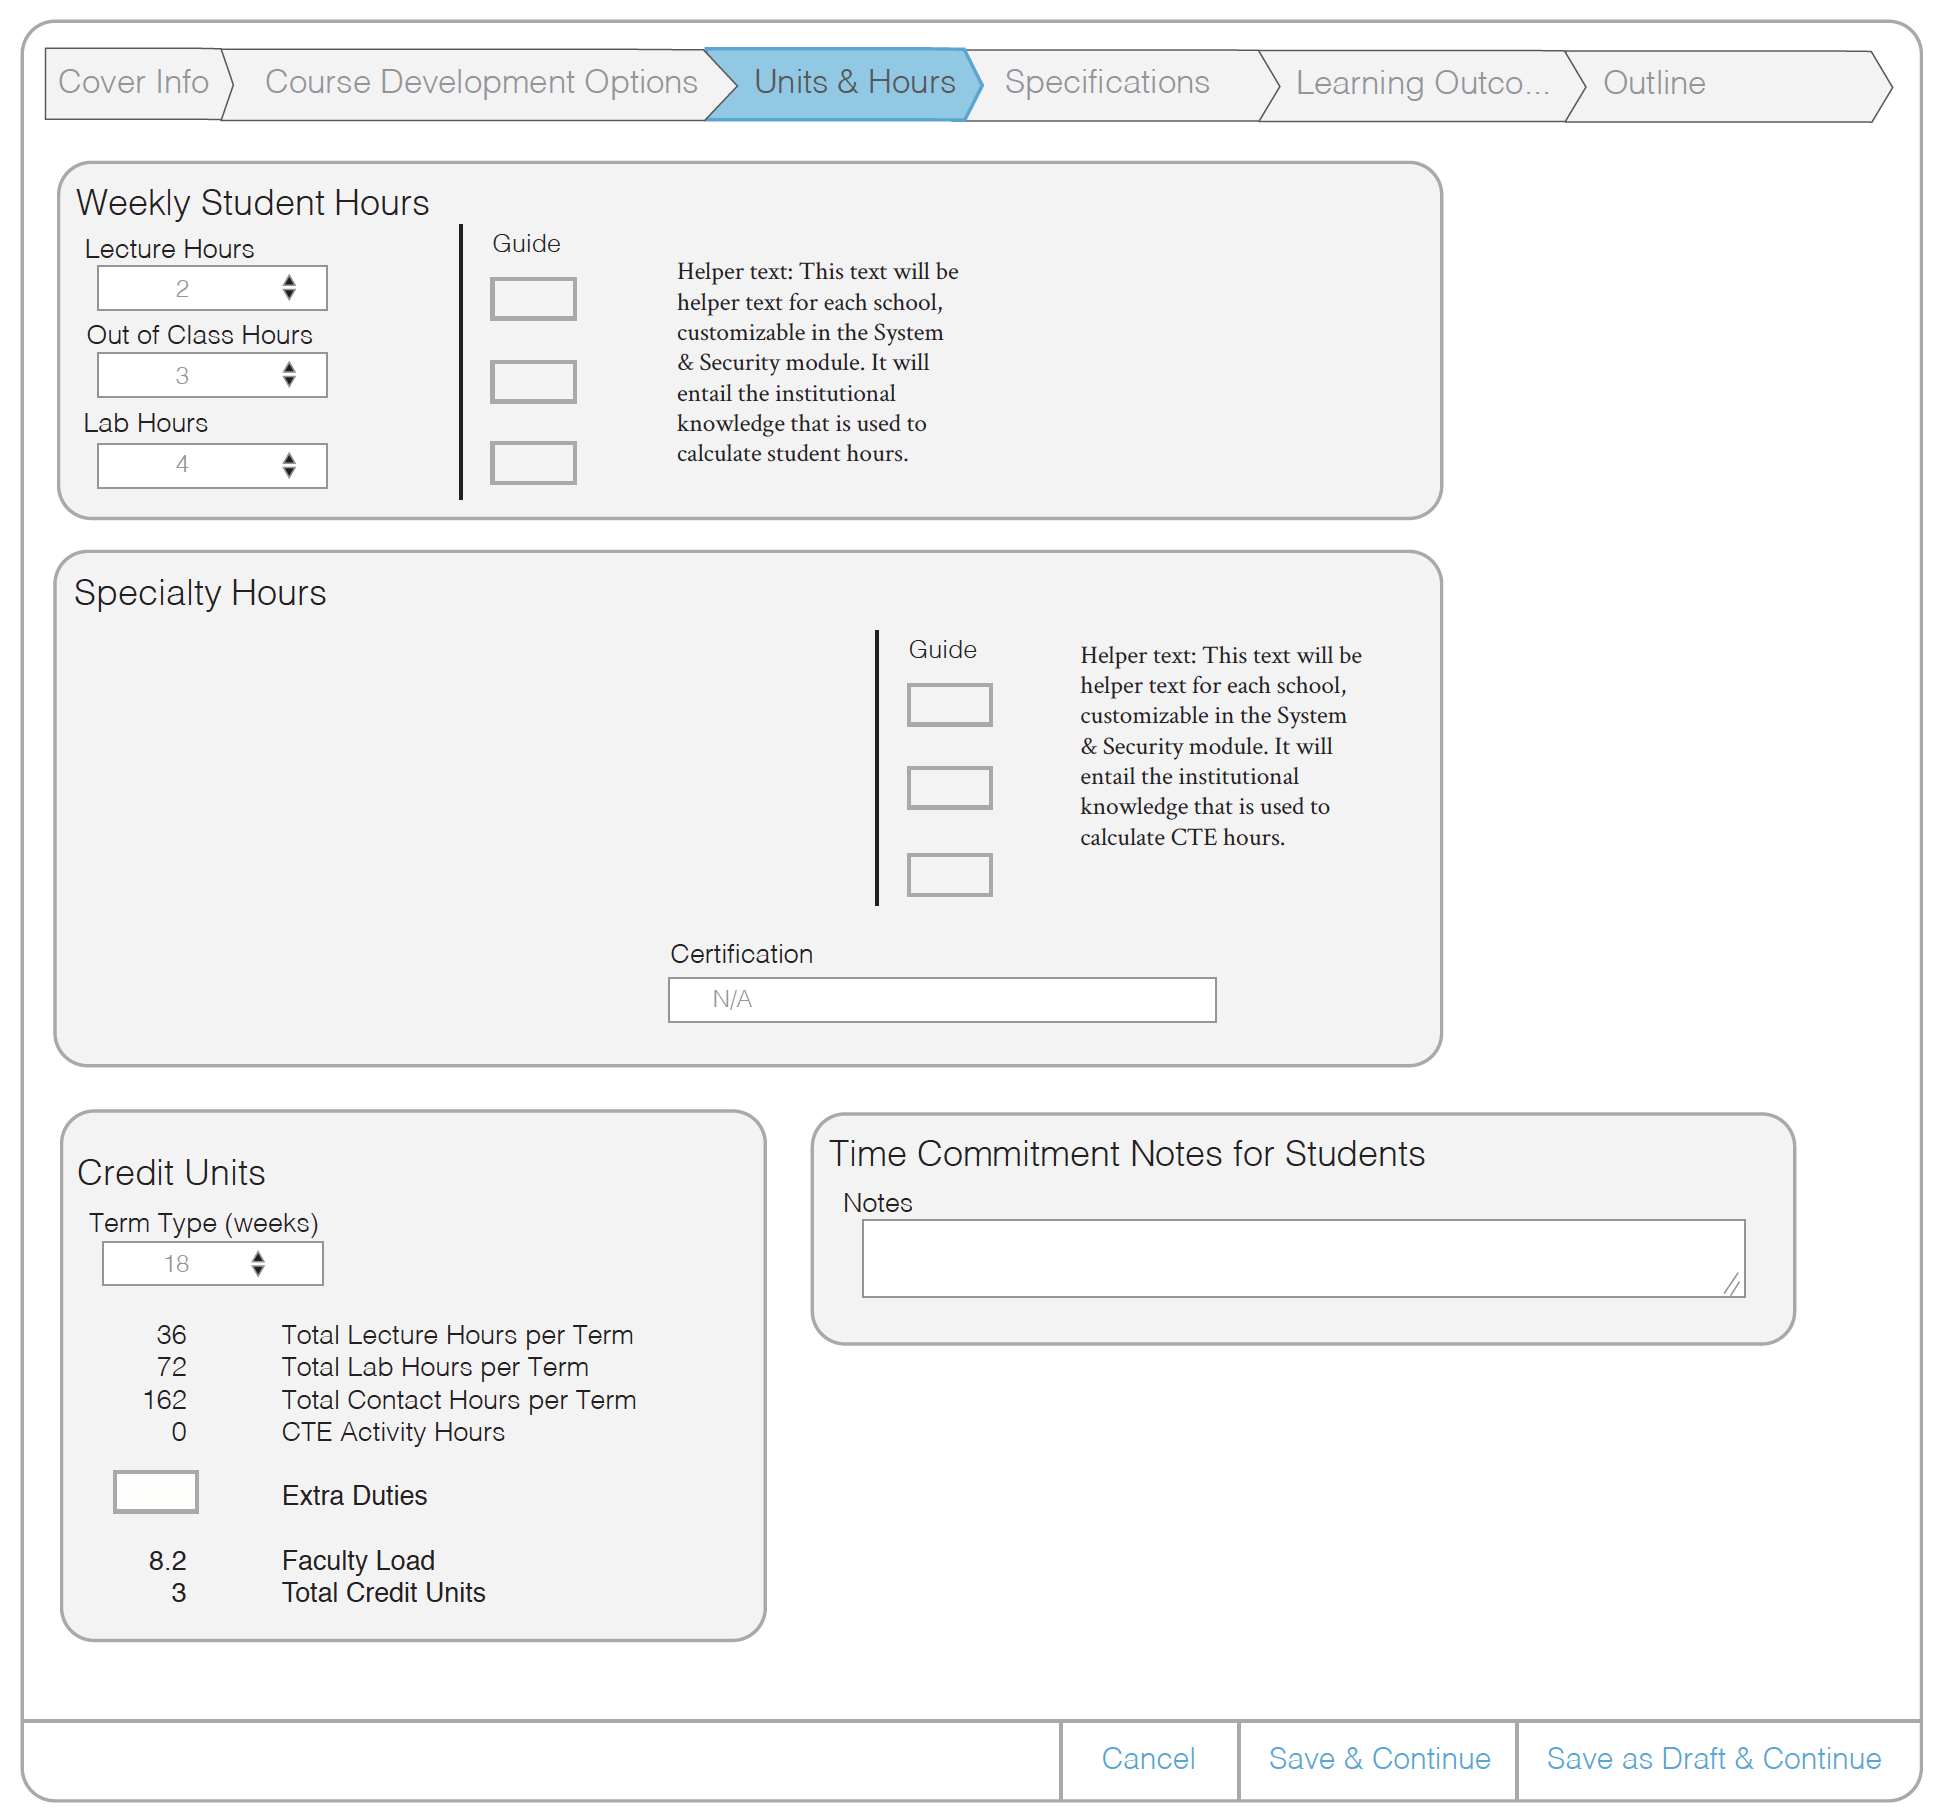
\includegraphics[scale=0.3]{Capitulos/DesarrollodelaAplicacion/Imagenes/course_units_hours}
\caption{Mockup de la pantalla de horas y unidades de evaluación de curso.}
  \label{course_units_hours}
\end{figure}

\subsection{Especificaciones de curso}
En la siguiente historia de usuario ha desarrollado un nuevo paso para el flujo de trabajo en la cual el encargado del flujo de trabajo puede agregar objetivos, información acerca de los métodos de evaluación de la materia, algunos equipos requeridos y libros que se necesitará en el curso.

Se han proporcionado de mockups (figura \ref{course_specs}) para el nuevo paso y era un criterio de aceptación de la historia de usuario seguir el mismo formato para el desarrollo de la misma.

La historia de usuario proporciona la siguiente descripción: \enquote{\textit{Como profesor encargado de curso, me gustaría ser capaz de agregar o editar especificaciones de curso como parte del flujo de trabajo de creación y/o versionamiento de mi curso para no tener que hacerlo en papel}}.

Las tareas fueron separadas y desarrolladas por los desarrolladores y eran las siguientes:
\begin{itemize}
	\item Migrar los datos para que soporte el nuevo formato de cursos.
	\item Crear y/o modificar clases de Java para el nuevo modelo de datos.
	\item Actualizar la página de plantillas de flujo de trabajo para que soporte el nuevo paso.
	\item Actualizar el visualizador de flujo de trabajo.
	\item Actualizar los servicios de guardado para creación y versionamiento de cursos y flujo de trabajos.
	\item Actualizar el servicio de aprobación de flujo de trabajo.
\end{itemize}

La historia fue terminada en una iteración con 40 horas de desarrollo cargadas en el sistema

\begin{figure}[H]
\centering
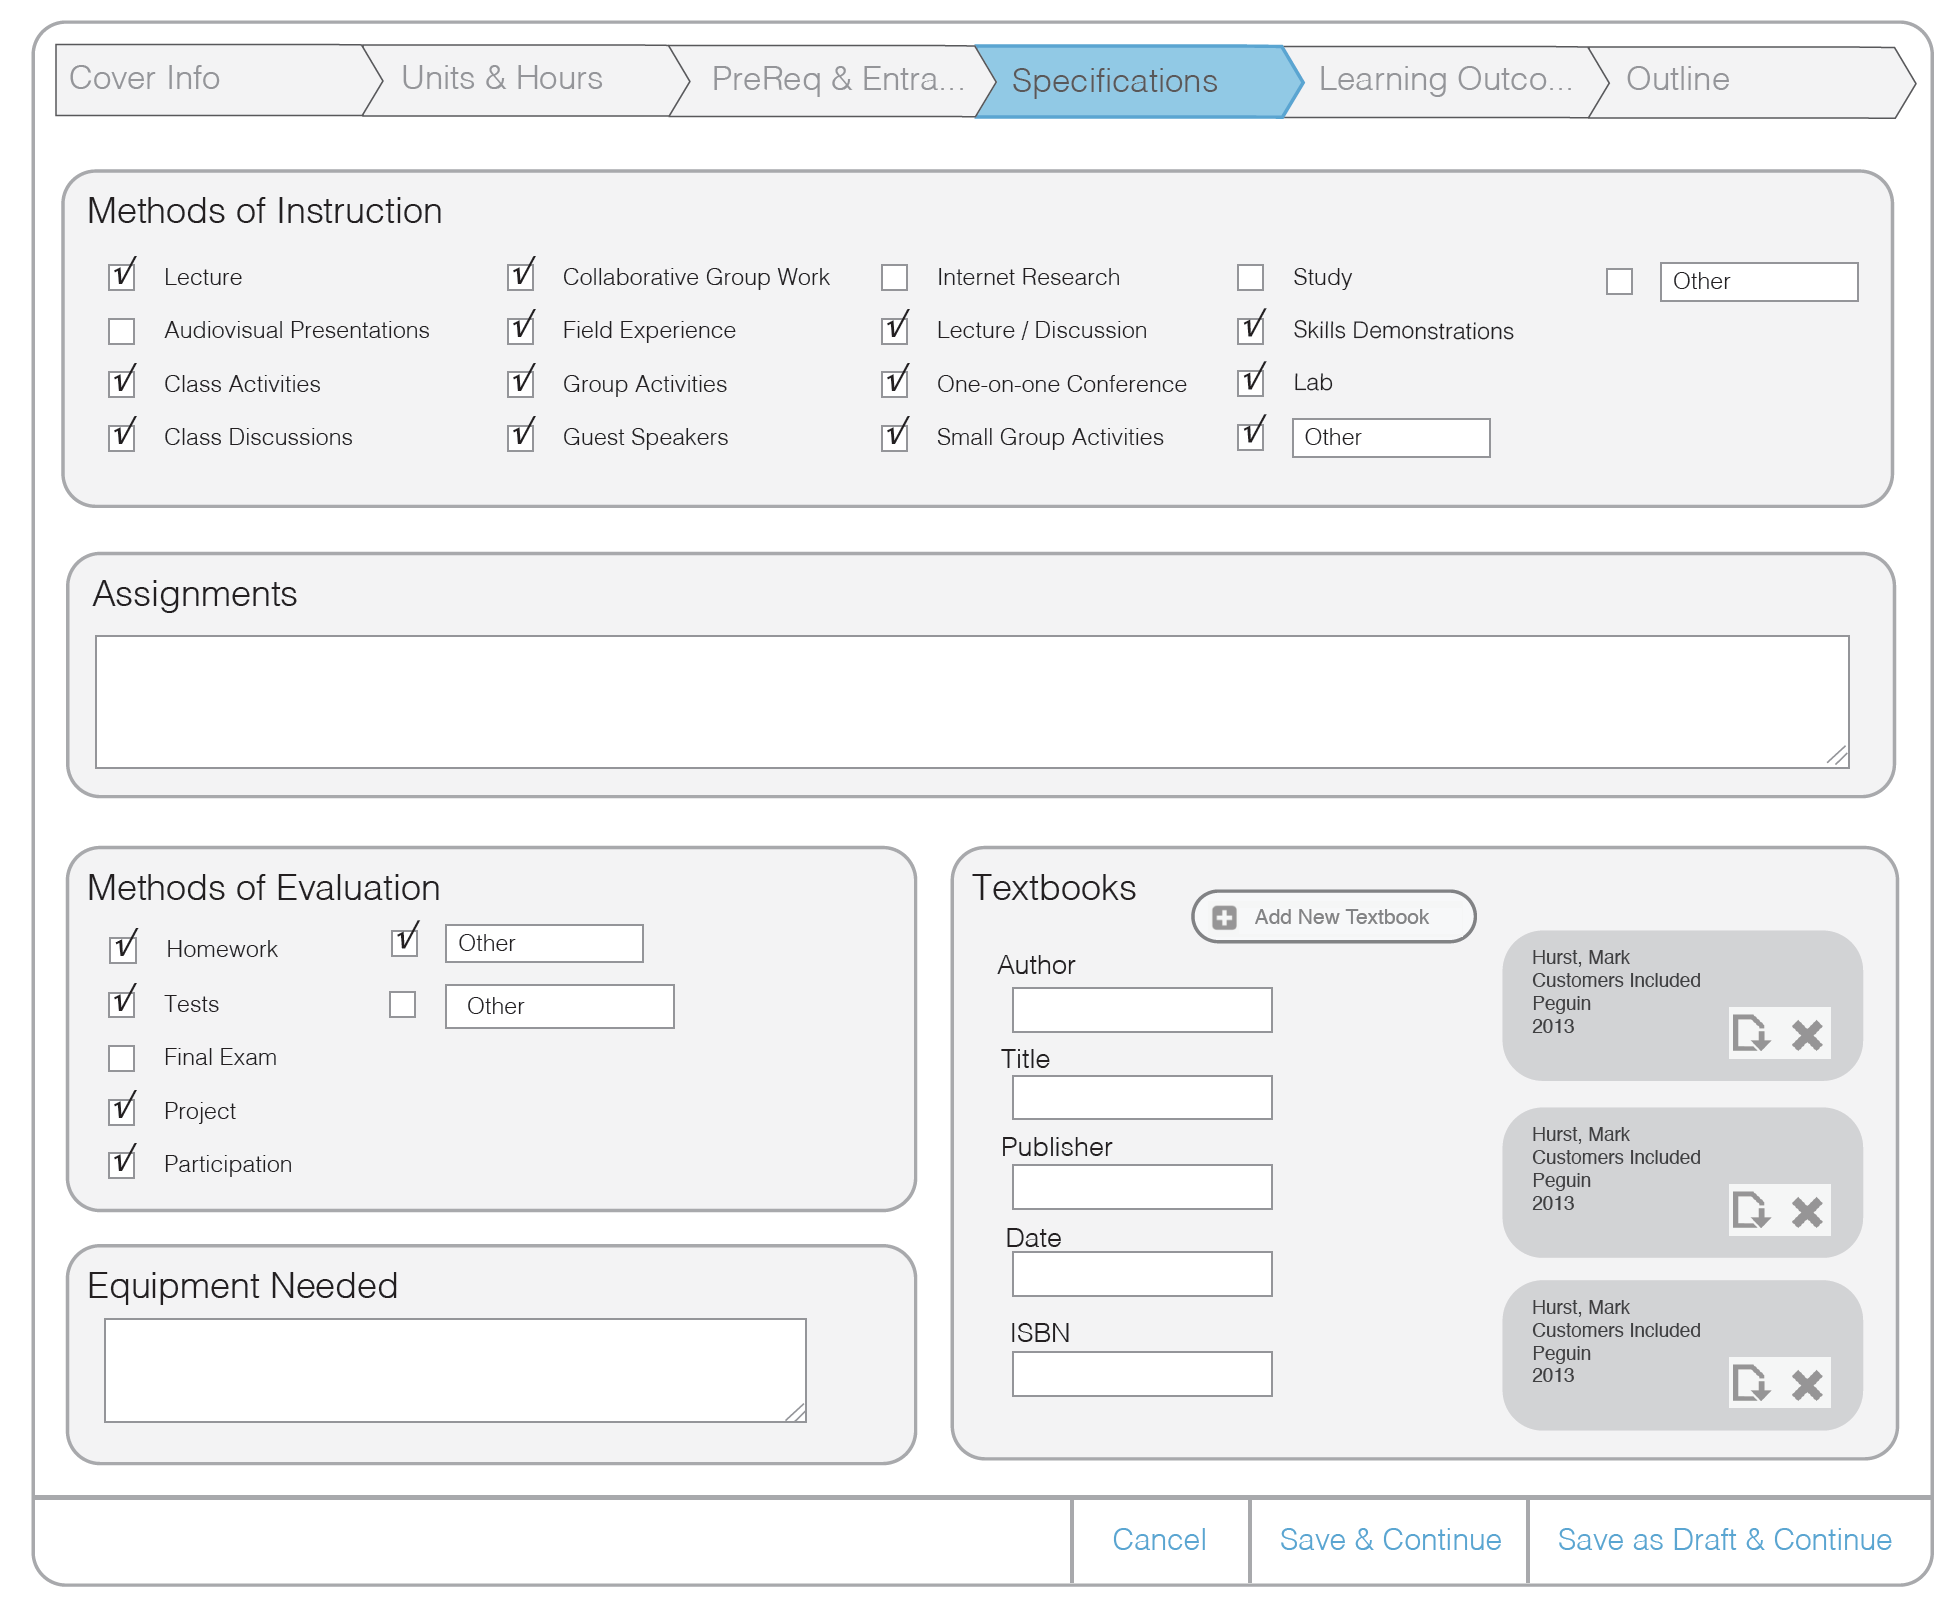
\includegraphics[scale=0.3]{Capitulos/DesarrollodelaAplicacion/Imagenes/course_specs}
\caption{Mockup de la pantalla de especificaciones de curso.}
  \label{course_specs}
\end{figure}

\subsection{Requisitos de curso}
Esta historia tiene como propósito el de adaptar el modelo de datos para que una lista de cursos como pre-requisitos, co-requisitos, anti-requisitos, y recomendaciones para su nuevo curso. Además, de ciertas capacidades que el alumno debe tener como requisito para tomar el curso.

Para entrar un poco en contexto de la historia vamos a definir cuáles son los tipos de requisitos que puede tener un curso:

\begin{itemize}
	\item \textbf{Pre-requisito:} es un tipo de requisito que impide al usuario tomar o cursar un curso sin haber aprobado antes del curso que está como pre-requisito.
	\item \textbf{Co-requisito:} es un tipo de requisito que impide al usuario tomar un curso si no cursa también el curso que tiene como co-requisito.
	\item \textbf{Anti-requisito:} es un requisito que impide al usuario tomar un curso si ya aprobó o va a tomar un curso que tiene como anti-requisito.
	\item \textbf{Recomendación:} es una recomendación por parte del sistema que materia tomar para aprovechar mejor la malla. Es opcional.
\end{itemize}

La historia de usuario tiene como descripción: \enquote{\textit{Como persona encargada de un curso, me gustaría ser capaz de introducir requisitos para cursos y ciertas competencias adquiridas en la creación o revisión de flujo de trabajo, para que podamos seguir durante su desarrollo y aprobación}} y la figura \ref{course_req} muestra mockups para la pantalla.

La historia fue dividida en partes para que los desarrolladores puedan trabajar en partes independientes durante el proceso de la misma, y eran las siguientes:
\begin{itemize}
	\item Diseñar y actualizar el modelo de datos atual.
	\item Generar y actualizar clases Java para la lógica.
	\item Actualizar la plantilla de flujo de trabajo para que soporte un nuevo paso.
	\item Actualizar el visualizador de flujo de trabajo.
	\item Actualizar los servicios de guardado y aprobación.
	\item Pruebas de funcionalidad.
\end{itemize}

La historia de usuario ha sido terminada en una iteración con 44 horas de desarrollo cargadas en el sistema.

\begin{figure}[H]
\centering
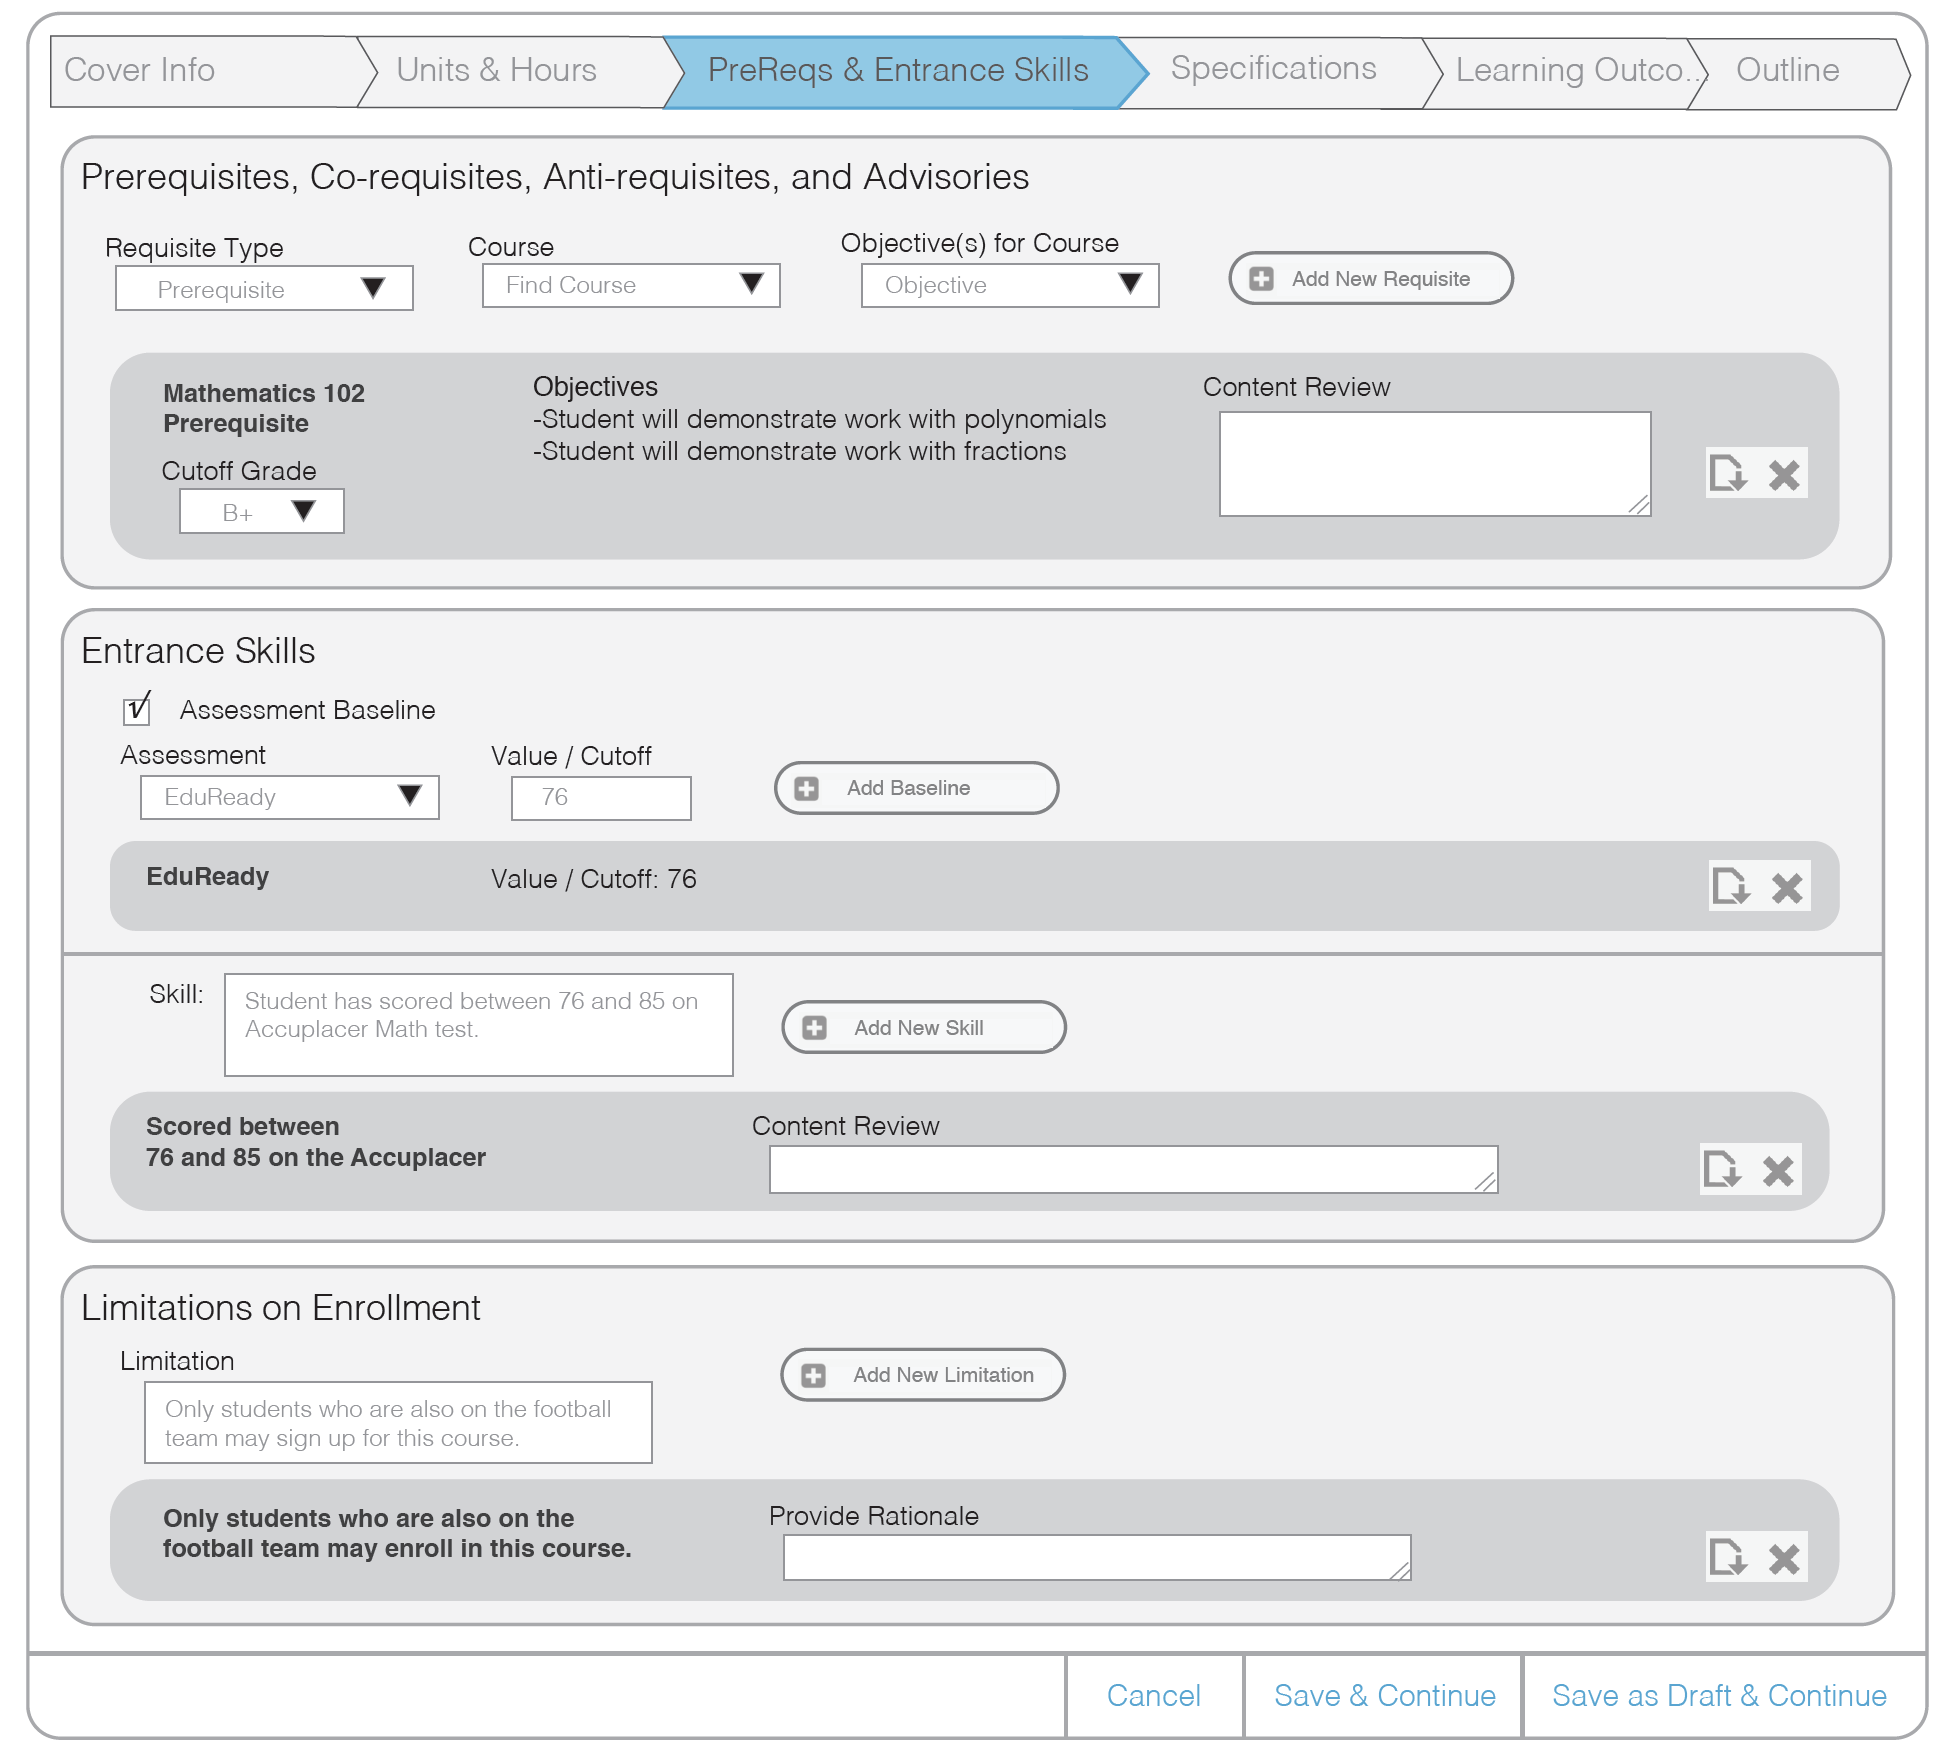
\includegraphics[scale=0.3]{Capitulos/DesarrollodelaAplicacion/Imagenes/course_req}
\caption{Mockup de la pantalla de requisitos de curso.}
  \label{course_req}
\end{figure}

\subsection{Revisar y aprobar curso}
La historia de usuario tiene como criterios de aceptación los siguientes puntos:
\begin{itemize}
	\item Las páginas para revisar los flujo de trabajos tienen una región de retroalimentación o feedback debajo de cada paso, con la opción de ocultar y mostrar para que el usuario que está revisando el flujo de trabajo en desarrollo pueda dejar comentarios al encargado del formulario del curso.
	\item La interfaz tiene elementos de estado que indican que cierta parte es nueva, aprobada, y rechazada.
	\item Los pasos tienen regiones que permiten aceptar o rechazar los campos propuestos por los desarrolladores del curso. Por lo tanto, deben tener elementos de interfaz que indiquen al usuario que puede aprobar o rechazar cada parte.
\end{itemize}
Además de los criterios de aceptación, había que volver a actualizar el buzón de entrada para que acepten los cambios que tiene la historia de usuario. Debido a que más de una persona puede revisar el flujo de trabajo y podría trancar el proceso si es que no se le notifica debidamente que hay nuevos cambios que revisar.

Algunas de las tareas descompuestas de la historia de usuario son las siguientes:
\begin{itemize}
	\item Actualizar el visualizador de flujo de trabajo para que pueda soportar la nueva característica de aprobación o rechazo de cada parte.
	\item Actualizar el buzón de entrada de Cursos.
	\item Pruebas de funcionamiento.
\end{itemize}

La historia se ha terminado en una iteración con 68 horas cargadas de desarrollo

\subsection{Competencias de curso}
Esta historia tiene como propósito de crear o versionar competencias para el curso a ser creado o versionado. 

La organización ha proporcionado mockups (figura \ref{course_learning_outcomes}) para el paso a desarrollarse y era un criterio de aceptación de parte del ticket que siga el mismo formato.

La historia de usuario tiene como descripción: \enquote{\textit{Como encargado del formulario de curso, me gustaría ser capaz de articular las competencias de mi nuevo curso, para de esa manera de tener que estar añadiendo una a una después de completar el proceso de creación de cursos con el flujo}}.

Como criterio de aceptación de la historia fue la de agregar el flujo de trabajo de competencias en el flujo de trabajo de cursos. Algunas de las tareas de la historia fueron:
\begin{itemize}
	\item Modificar la base de datos para que soporte el nuevo modelo de datos de las competencias dentro de flujo de trabajo de curso.
	\item Modificar o agregar clases de las entidades que van a ser usadas durante la historia.
	\item Actualizar la plantilla de flujo de trabajo para que soporte el nuevo paso para la creación o versionamiento de competencias.
	\item Actualizar el visualizador de flujo de trabajo para que soporte el nuevo paso de competencias.
	\item Actualizar los servicios de guardado y de versionamiento de cursos y competencias.
	\item Pruebas de nuevas funcionalidades.
\end{itemize}

La historia ha sido terminada en dos iteraciones con un total de 76 horas cargadas en el sistema.

\begin{figure}[H]
\centering
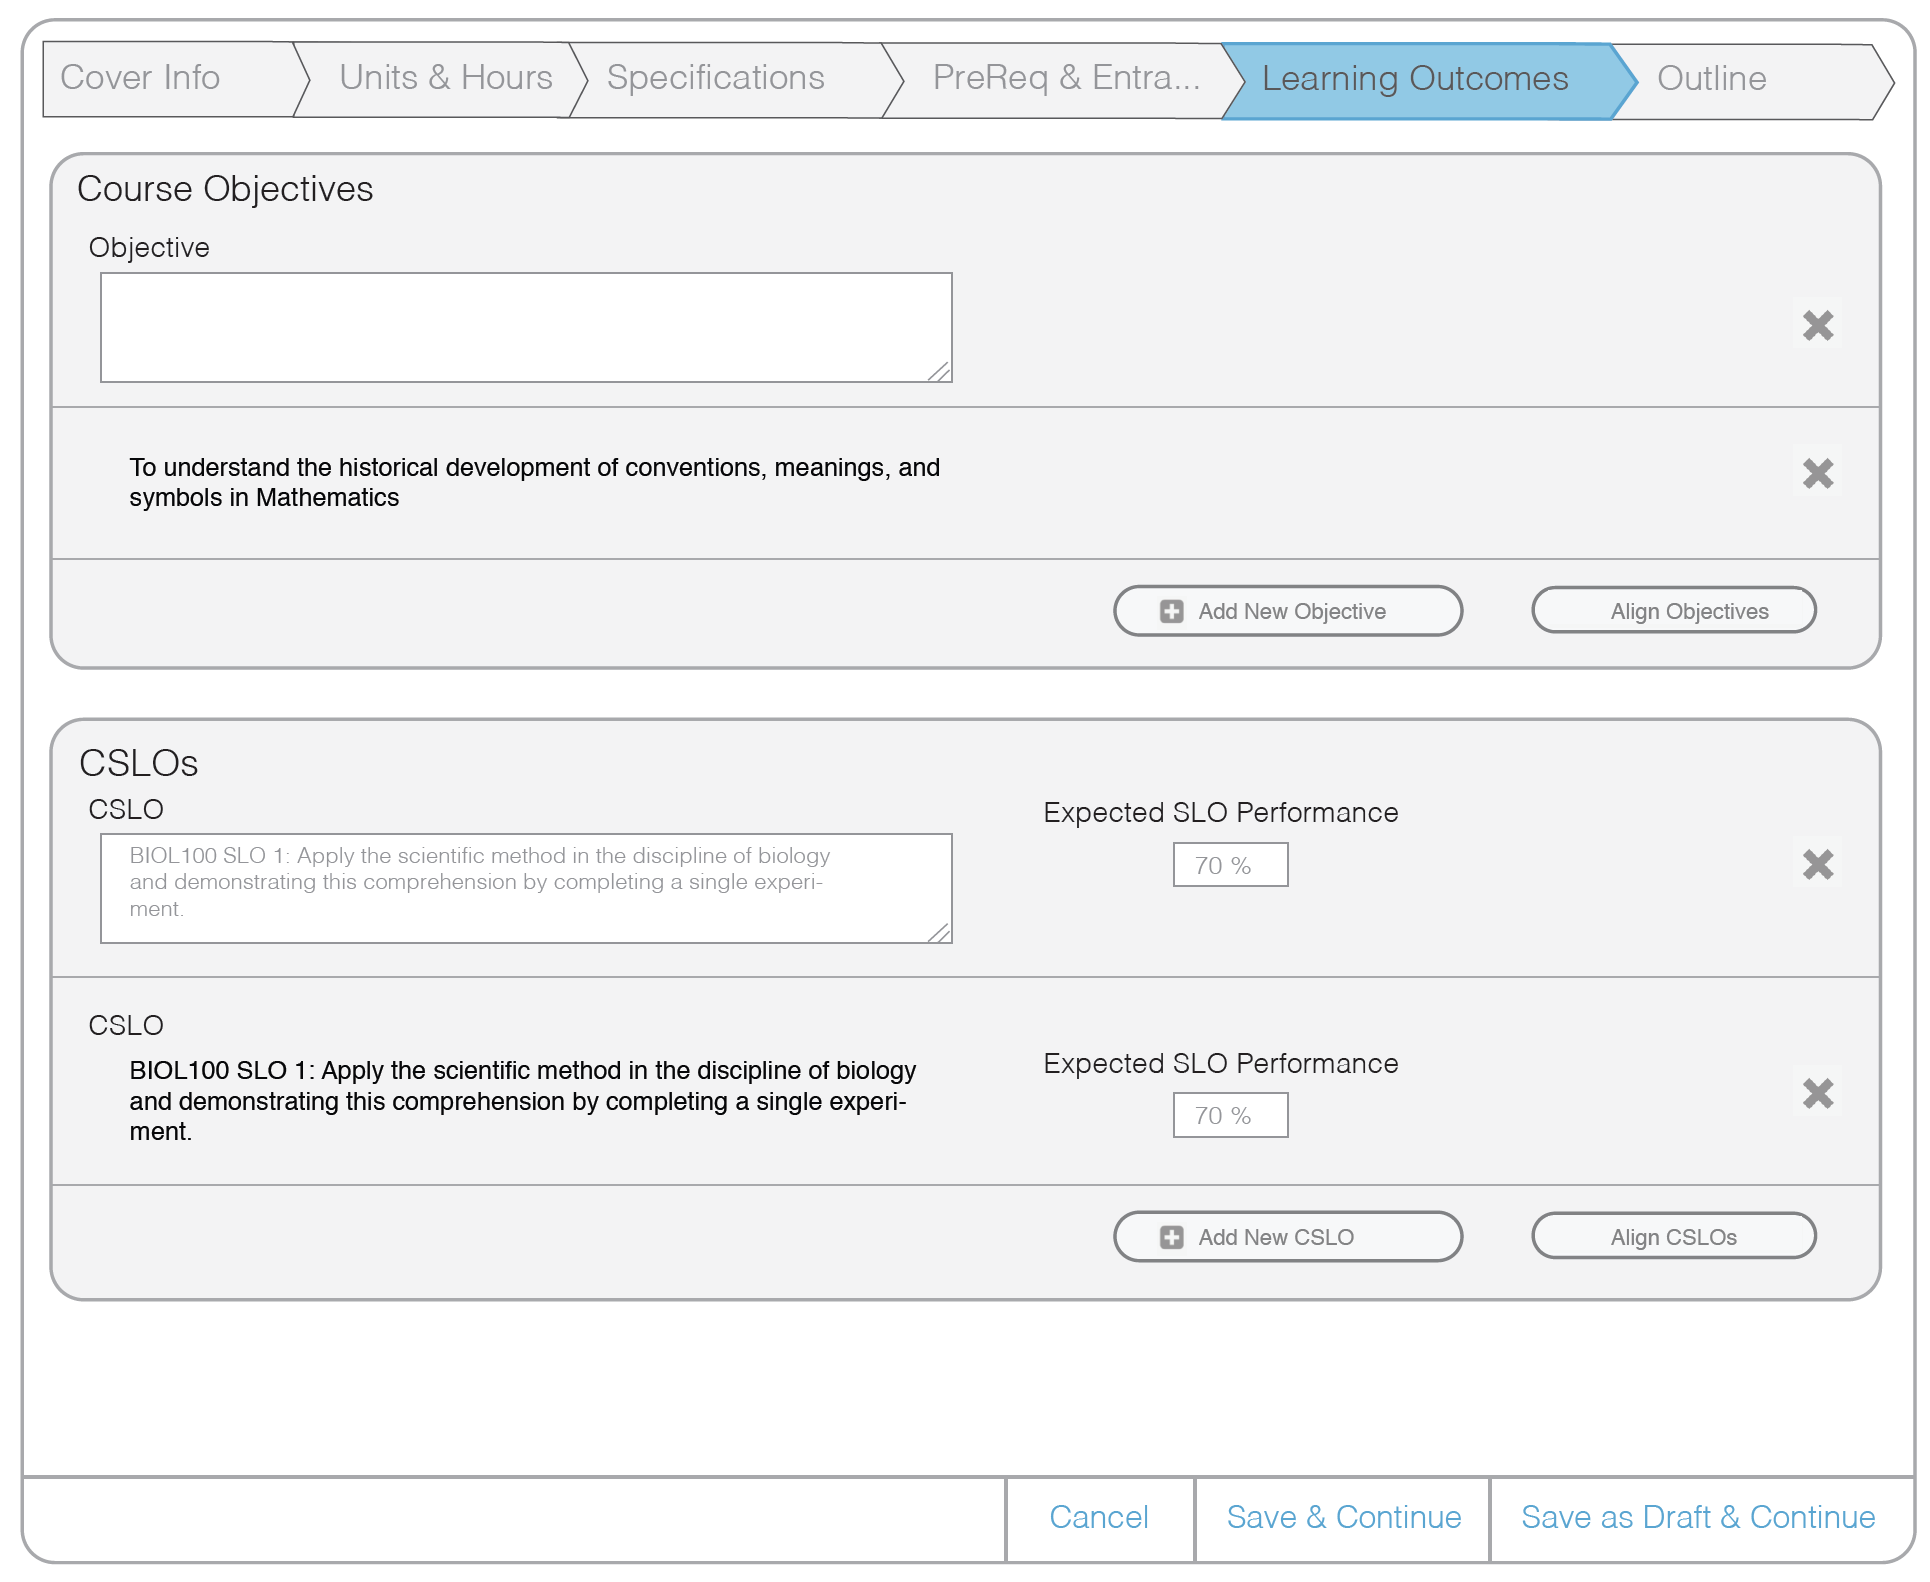
\includegraphics[scale=0.3]{Capitulos/DesarrollodelaAplicacion/Imagenes/course_learning_outcomes}
\caption{Mockup de la pantalla de competencias de curso.}
  \label{course_learning_outcomes}
\end{figure}

\subsection{Esquema de curso}
Esta historia tiene como propósito de diseñar la pantalla para un nuevo paso para el flujo de trabajo. 

La organización ha proporcionado mockups (figura \ref{course_outline}) para el paso a desarrollarse y era un criterio de aceptación de parte del ticket que siga el mismo formato.

La historia de usuario tiene como descripción: \enquote{\textit{Como encargado del formulario de curso, me gustaría ser capaz de agregar el esquema de un curso, para de esta manera dar un resúmen de curso para el que esté revisando mi flujo y para que los estudiantes puedan tener una idea de se trata una vez que se curse}}.

Como criterio de aceptación de la historia fue la de agregar el flujo de trabajo de competencias en el flujo de trabajo de cursos. Algunas de las tareas de la historia fueron:
\begin{itemize}
	\item Modificar la base de datos donde se tendría que almacenar los nuevos campos de esquema ya sea para el curso y para el flujo que se desarrolla.
	\item Modificar o agregar clases de las entidades que van a ser usadas durante la historia.
	\item Actualizar la plantilla de flujo de trabajo para que soporte el nuevo paso de esquema de cursos.
	\item Actualizar el visualizador de flujo de trabajo para que soporte el nuevo paso de competencias.
	\item Actualizar los servicios de guardado y de revisión para que soporte nuevo paso.
\end{itemize}

La historia ha sido terminada en dos iteraciones con un total de 48 horas cargadas en el sistema.

\begin{figure}[H]
\centering
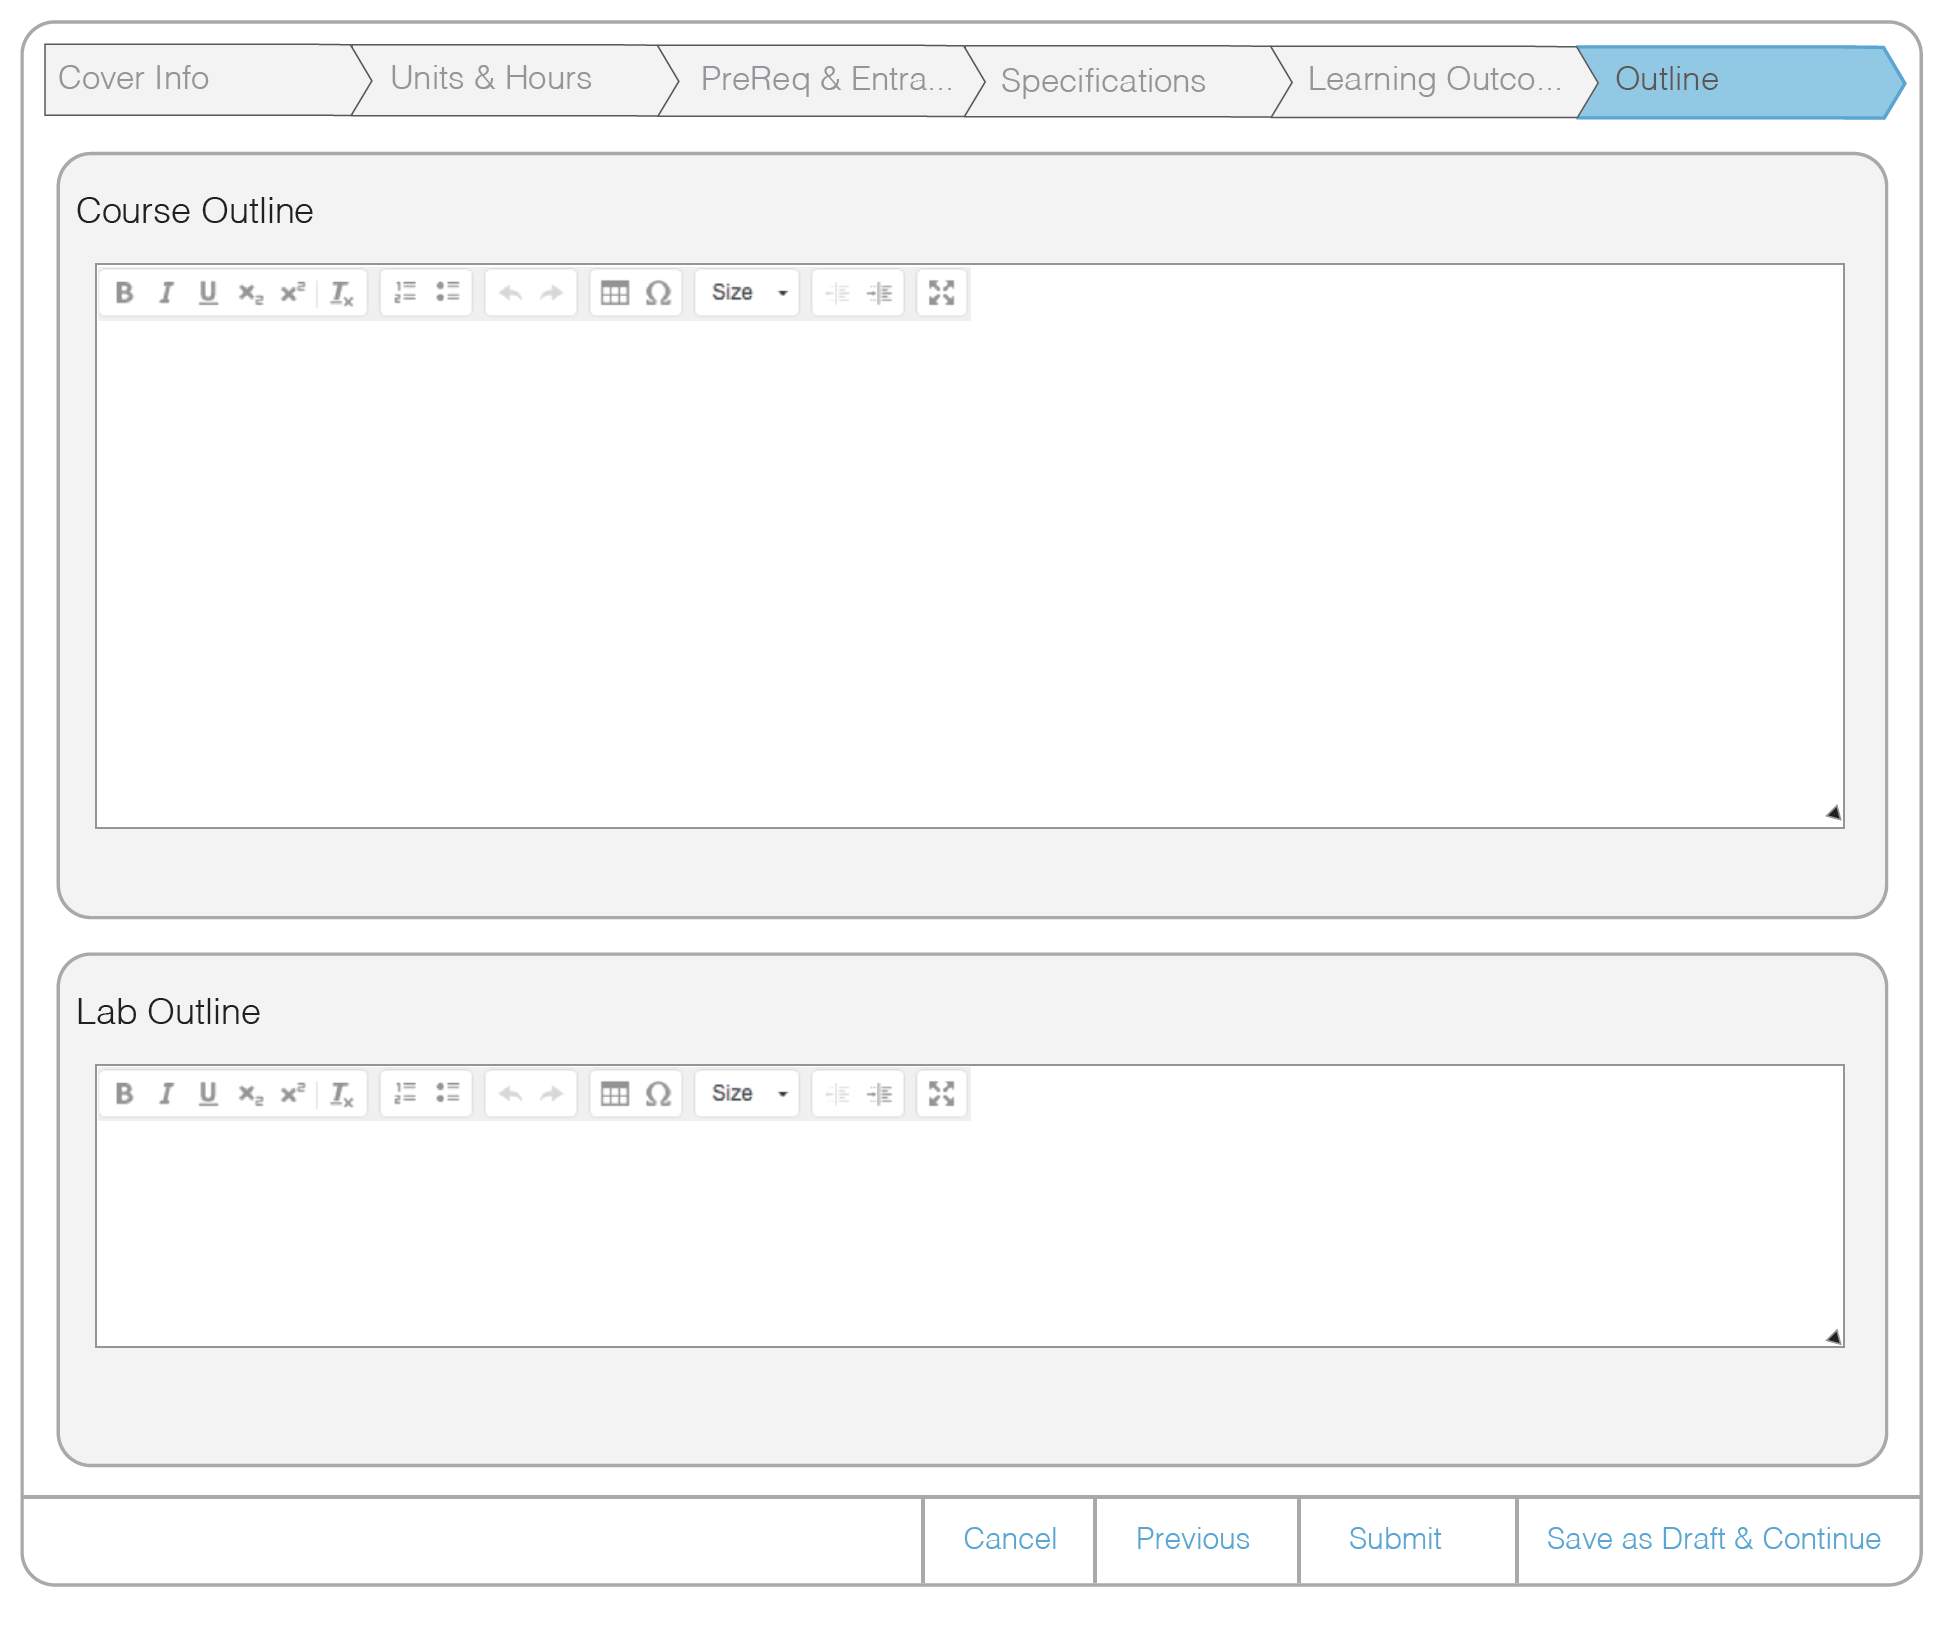
\includegraphics[scale=0.3]{Capitulos/DesarrollodelaAplicacion/Imagenes/course_outline}
\caption{Mockup de la pantalla de esquema de curso.}
  \label{course_outline}
\end{figure}

\subsection{Codigos de clasificación de curso}
La siguiente historia tiene como propósito la de asignar códigos de clasificación a los cursos.

Para entrar en contexto, habría que definir primero que es TOP\footnote{de sus siglas en inglés, Taxonomy Of Programs, que significa en español taxonomía de programas.}.

TOP es un sistema numérico de códigos usados a nivel de Estado para recolectar y reportar información en cursos y programas, en diferentes instituciones educativas \citep{brice_w_harris_program_2013} por todo el Estado. 

Ha sido diseñado para agregar información acerca de los programas. Sin embargo, un código TOP debe ser asignado a cada curso del sistema. 

Aunque no contiene tantas opciones específicas como lo haría un sistema diseñado para cursos, a cada curso se le debe dar el código que se aproxima a describir el contenido del curso.

Algunos usos a los códigos:
\begin{itemize}
	\item En el inventario de programas aprobados y rechazados, para tener información que tipos de cursos y programas son ofrecidas por el estado.
	\item En bases de datos de administración de información, para recolectar y reportar información en logros estudiantiles (licenciaturas y certificados) en ciertos programas.
	\item En contabilidad vocacional estudiantil, para reportes de compleción de programas y cursos de ciertos programas vocacionales.
\end{itemize}

La descripción de la historia fue la siguiente: \enquote{\textit{Como miembro del comité curricular, me gustaría ser capaz de asignar a mis cursos de códigos de clasificación como parte de la aprobación de mis flujo de trabajos para asegurar que estén correctos, como esto es motivo de rechazo en la oficina del canciller del Estado}}.

Algunas de las tareas fueron las siguientes:
\begin{itemize}
	\item Diseño del nuevo modelo, donde se debían generar tablas para cada nueva entidad del modelo de datos ajustado para las taxonomías de programas. Además, cargar todos los datos de códigos de cursos existentes para el estado de California.
	\item Creación de clases Java.
	\item Diseño e implementación páginas CRUD para disciplina, sub-disciplina, y campo.
	\item Diseño e implementación de la nueva página de asignación de códigos de clasificación para los cursos en proceso de diseño.
	\item Hacer servicios para cada una de las nuevas páginas.
	\item Pruebas de funcionalidad.
\end{itemize}

La historia de usuarioha sido terminada en una iteración con 80 horas cargadas en el sistema.


[VER SI TIENE MOCKUP]